\chapter{Introdução}

Esta seção visa introduzir o(a) leitor(a) aos principais temas deste trabalho. São apresentados conceitos introdutórios sobre testes automatizados de aplicações web e sobre o teste de mutação como forma de avaliar a eficácia de suítes de testes. Além disso, são apresentados o delineamento do problema, a questão de pesquisa norteadora desta investigação e os objetivos do trabalho. Por fim, são apresentadas a estrutura do trabalho e o cronograma de atividades, dividido em duas etapas.

\section{Contexto}

A qualidade de software constitui um aspecto fundamental no desenvolvimento e na manutenção de sistemas computacionais, especialmente diante da crescente complexidade das aplicações e da necessidade de garantir seu funcionamento adequado em diferentes cenários de utilização \cite{kochhar2015code}.

Nesse contexto, os testes de software desempenham um papel central na identificação de defeitos, na verificação do comportamento esperado e na redução dos riscos associados à entrega de produtos que não atendam aos requisitos estabelecidos. Com a ampliação da utilização de práticas de desenvolvimento ágil e integração contínua, os testes automatizados passaram a ser essenciais no desenvolvimento moderno de aplicações web, sendo amplamente empregados para validar funcionalidades sob a perspectiva do usuário, sobretudo por meio de testes de regressão e testes de ponta a ponta (end-to-end) \cite{yandrapally2021}.


Apesar dos benefícios proporcionados pela automação, a existência de uma suíte de testes não representa, por si só, uma garantia de que o software esteja livre de defeitos. Uma suíte pode executar todos os seus casos sem apresentar falhas e, ainda assim, não possuir verificações capazes de identificar alterações indesejadas no comportamento da aplicação. Tradicionalmente, a qualidade e a abrangência desses testes são medidas por meio de métricas de cobertura de código \cite{zhang2022}.

Embora indiquem quais linhas ou ramos foram executados durante a suíte, a execução de uma instrução não implica necessariamente que o comportamento produzido tenha sido efetivamente validado por asserções. Essa limitação motiva diversas investigações sobre a correlação entre métricas tradicionais e a eficácia real dos testes. \citeonline{assylbekov2013} investigaram a relação entre o mutation score e as métricas de cobertura de código, enquanto  \citeonline{alenezi2016} sugerem que o uso conjunto e comparativo de ambas as abordagens oferece um panorama mais robusto sobre a qualidade dos testes.

Nesse cenário, os testes de mutação consolidam-se como uma técnica rigorosa para avaliar a capacidade de uma suíte de revelar defeitos. O procedimento consiste em inserir pequenas falhas artificiais no código-fonte, denominadas mutantes, por meio de operadores de mutação específicos \cite{guerino2024}. A suíte de testes é executada sobre esses programas modificados: o mutante é considerado "morto" quando ao menos um teste falha, e "sobrevivente" quando todos passam. O mutation score, razão entre mutantes mortos e o total de mutantes válidos, serve como evidência da capacidade da suíte em expor defeitos reais \cite{just2014}.

Embora robusta, a interpretação da técnica exige cautela. Fenômenos como a presença de mutantes equivalentes (que alteram a sintaxe mas preservam o comportamento) e mutantes teimosos exigem análises detalhadas acerca de alcance, infecção e propagação \cite{yao2014}. Além disso, embora \citeonline{just2014} tenham demonstrado que a detecção de mutantes possui forte correlação com falhas reais, superando a cobertura de comandos, cerca de 17\% das falhas reais não se acoplam a nenhum mutante, indicando os limites da técnica como substituta integral de defeitos em produção. Adicionalmente, desafios operacionais como o custo computacional exigem estratégias de otimização e redução do conjunto de mutantes \cite{kintis2010, guizzo2022}.

Apesar desses desafios, há fortes evidências do valor prático dessa técnica. Em um estudo longitudinal de seis anos no Google envolvendo cerca de 15 milhões de mutantes, constatou-se que desenvolvedores expostos à análise de mutação passaram a escrever mais testes e mais robustos, sendo que 70\% dos bugs de alta prioridade analisados apresentavam ao menos um mutante acoplado \cite{petrovic2021}.

No contexto específico de aplicações web, \citeonline{yandrapally2021} investigaram a utilização da análise de mutação para avaliar testes end-to-end, propondo a ferramenta MAEWU, que aplica 16 operadores de mutação derivados da análise de 250 relatos de bugs ao DOM dinâmico do navegador. Contudo, a RSL realizada neste trabalho, consolidando 36 estudos publicados entre 2010 e 2026, com predominância de ferramentas voltadas à linguagem Java, como MuJava e PIT, além de Major e Proteum, aponta que a literatura sobre o uso de testes de mutação para avaliar suítes de aplicações web ainda é escassa. Esse descompasso entre a relevância das aplicações web modernas e a restrição de pesquisas na área evidencia a necessidade de investigações aprofundadas sobre a aplicabilidade e eficácia dos testes de mutação nesse domínio.

\section{Problema}

Apesar da ampla adoção de suítes automatizadas, a obtenção de resultados positivos e de alta cobertura de código não garante, por si só, que o software esteja livre de defeitos. A aprovação dos testes depende da presença de oracluos capazes de perceber comportamentos incorretos, o que evidencia a carência de um método consolidado para aferir a eficácia de suítes voltadas a aplicações web \cite{yandrapally2021}. 

Além disso, a aplicação de testes de mutação para mitigar essa lacuna esbarra em obstáculos práticos significativos. Conforme apontado na RSL deste trabalho, o custo computacional e o esforço humano figuram como limitações em cerca de dois terços dos estudos, enquanto a gestão de mutantes equivalentes, que mantêm a semântica do programa e exigem frequentes análises manuais, afeta pouco mais da metade \cite{yao2014}. A interpretação torna-se ainda mais complexa ao distinguir se um mutante sobrevivente é equivalente, fruto de inadequação da suíte ou um mutante "teimoso" \cite{yao2014}.

Soma-se a isso o fato de que a técnica possui fronteiras intrínsecas: nem todas as falhas reais encontram correspondência direta nos mutantes gerados \cite{just2014}. Equipes de desenvolvimento e pesquisadores enfrentam, portanto, o desafio de medir com precisão a eficácia de testes em aplicações web, levanbdo em conta custo, operadores, ferramentas e a ambiguidade dos mutantes sobreviventes.

Dessa forma, o problema central investigado neste trabalho consiste em saber como avaliar de forma fundamentada e viável a eficácia de suítes de testes automatizados em aplicações web, considerando os limites operacionais e interpretativos da análise de mutação.

\section{Questão de Pesquisa}

Para definir a questão de pesquisa norteadora deste trabalho foi utilizada a abordagem Goal Question Metric (GQM), que propõe a especificação hierárquica de objetivos, questões e métricas de maneira top-down \cite{basili1994}. O propósito dessa abordagem é transformar o planejamento e a mensuração dos objetivos de uma pesquisa em questões e métricas que embasem suas respostas. Adaptando essa estrutura ao contexto desta pesquisa, definiram-se as seguintes características: objeto de análise, propósito, foco, ponto de vista e contexto (vide \hyperref[tab:gqm-adaptado]{Tabela~\ref*{tab:gqm-adaptado}}).

\begin{table}[H]
    \centering
    \caption{GQM Adaptado}
    \label{tab:gqm-adaptado}
    \begin{tabular}{|l|p{10cm}|}
        \hline
        \textbf{Características} & \textbf{Valor} \\
        \hline
        Analisar & Suíte de testes automatizados \\
        \hline
        Propósito & Avaliar a versão do código-fonte gerada após a aplicação dos testes mutantes \\
        \hline
        Foco & Eficácia da suíte de testes na detecção de defeitos \\
        \hline
        Ponto de Vista & Pesquisador \\
        \hline
        Contexto & Aplicações web disponíveis em repositórios de código-fonte aberto \\
        \hline
    \end{tabular}
    \fonte{Adaptado de \citeonline{basili1994}.}
\end{table}

Considerando essa perspectiva definimos a seguinte questão principal de pesquisa deste estudo:

\textit{\textbf{Como avaliar a eficácia de uma suíte de testes automatizados na detecção de defeitos de aplicações web por meio de testes de mutação?}}

\begin{figure}[H]
    \centering
    \caption{Estrutura do Modelo GQM}
    \label{fig:exemplo}
    \fbox{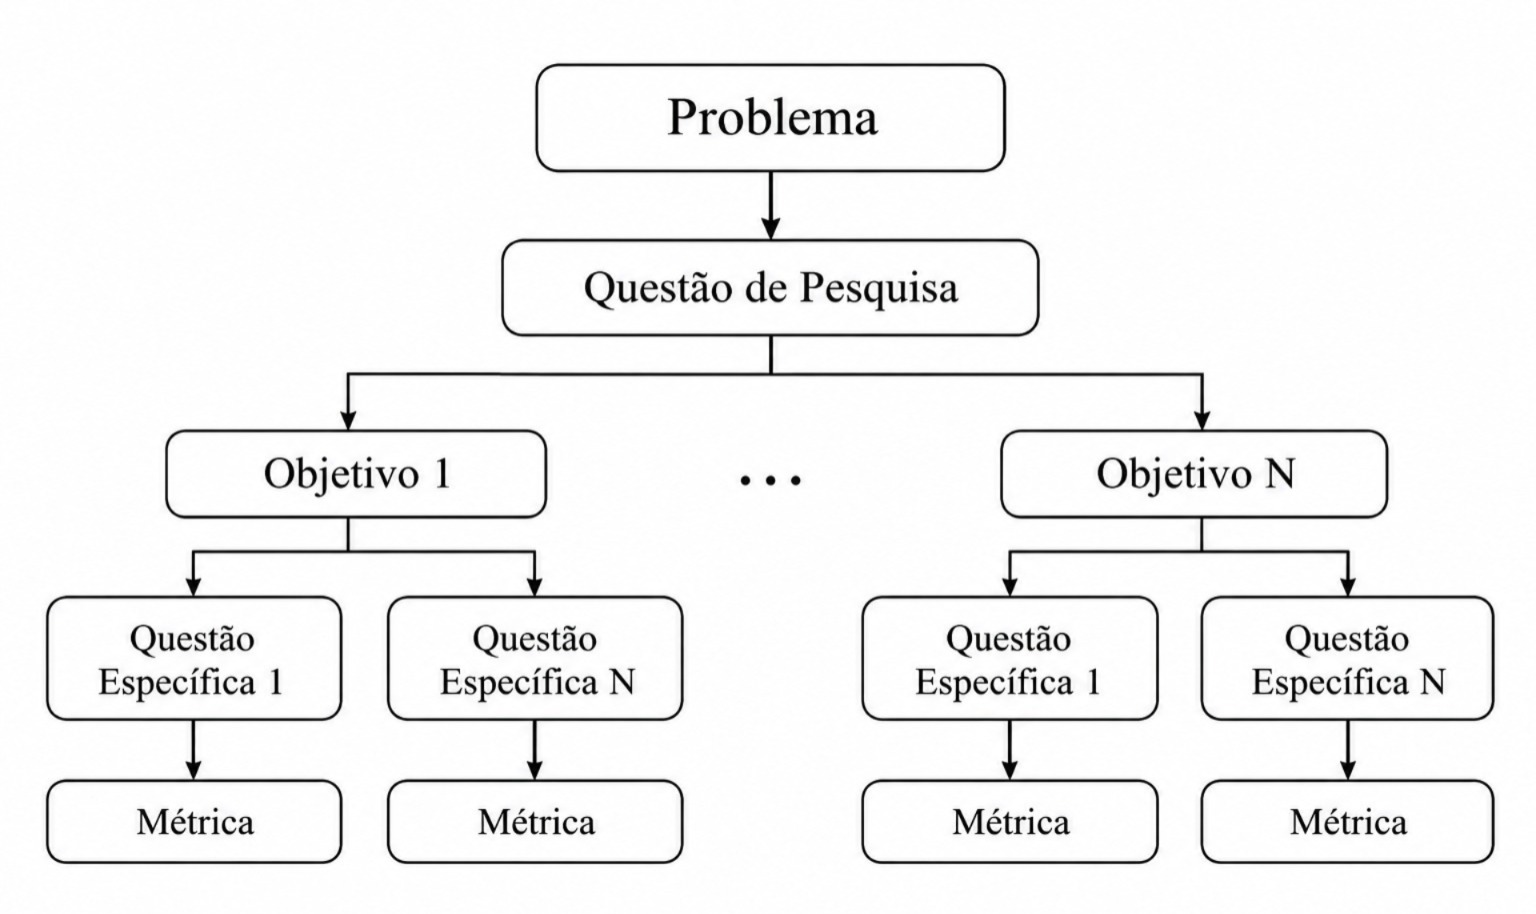
\includegraphics[width=0.8\textwidth]{figuras/GQM.png}}
    \vspace{0.2cm}
    \fonte{Adaptado de \citeonline{basili1994}.}
\end{figure}

A partir dessa questão foram definidas dez questões secundárias (SQ1 a SQ10), que orientam a revisão estruturada da literatura e são apresentadas no Capítulo~\ref{cap:revisao-literatura}, juntamente com a estratégia PICO utilizada na estruturação da busca.

\section{Objetivos}

O objetivo geral é investigar como avaliar a eficácia de suítes de testes automatizados na detecção de defeitos em aplicações web de código aberto por meio de testes de mutação, com base nas evidências reunidas pela RSL.
Para alcançar esse objetivo geral, foram definidos os seguintes objetivos específicos, que guiam as duas etapas deste trabalho:
\begin{itemize}

    \item Identificar, por meio de uma Revisão Sistemática da Literatura, as principais métricas utilizadas para avaliar a eficácia de suítes de testes automatizadas por meio de testes de mutação.
    
    \item Investigar os operadores de mutação, os tipos de mutantes e as ferramentas utilizados na avaliação de suítes de testes, considerando sua aplicabilidade ao contexto de aplicações web.
    
    \item Identificar as principais limitações, os custos computacionais e os desafios relacionados à aplicação de testes de mutação.
    
    \item Definir um procedimento experimental para avaliar a eficácia de suítes de testes automatizadas em aplicações web de código aberto, utilizando testes de mutação.
    
    \item Aplicar a análise de mutação nas aplicações selecionadas, registrando os resultados da execução das suítes de testes sobre os mutantes gerados.
    
    \item Analisar os resultados obtidos por meio de métricas como Mutation Score, quantidade de mutantes mortos e sobreviventes, cobertura de código e tempo de execução.
    
    \item Investigar os fatores associados à sobrevivência dos mutantes, considerando a possibilidade de equivalência e a capacidade da suíte de identificar as alterações introduzidas.
    
    \item Avaliar as contribuições e as limitações da utilização de testes de mutação como mecanismo de avaliação da eficácia de suítes automatizadas em aplicações web.
 
\end{itemize}

\section{Metodologia}
\label{sec:metodologia}

Esta subseção visa apresentar a metodologia adotada neste trabalho. Para descrevê-la, utiliza-se a estrutura de tomada de decisão para a escolha de um desenho de pesquisa em Engenharia de Software empírica proposta por \citeonline{wohlin2015}, apresentada na Figura~\ref{fig:exemplo2}. A estrutura parte da questão de pesquisa e organiza as decisões em três fases: a estratégica, que define o resultado, a lógica, o propósito e a abordagem da pesquisa; a tática, que define o processo e a metodologia de pesquisa; e a operacional, que define os métodos de coleta e de análise de dados e conduz aos resultados da pesquisa.

\begin{figure}[H]
    \centering
    \caption{Estrutura de tomada de decisão de pesquisa}
    \label{fig:exemplo2}
    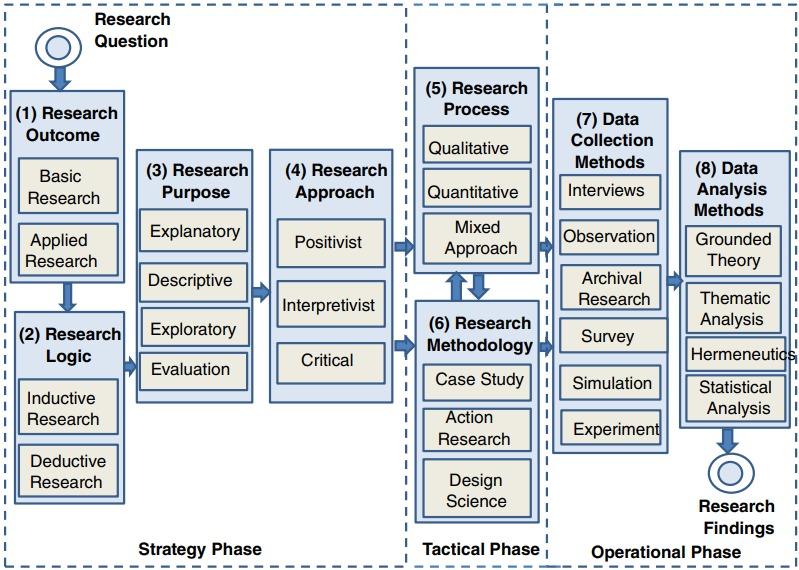
\includegraphics[width=0.8\textwidth]{figuras/estrutura-pesquisa.png}
\end{figure}
  \fonte{\citeonline{wohlin2015}.}

Na fase estratégica, define-se o resultado esperado, a lógica, o propósito e a abordagem. Quanto ao resultado, trata-se de uma pesquisa aplicada, pois busca resolver um problema prático: saber se os testes automatizados de uma aplicação web detectam falhas. Quanto à lógica, a primeira etapa é indutiva, pois a solução é construída a partir das evidências reunidas pela RSL, e a segunda é dedutiva, pois a solução definida é aplicada a aplicações web de código aberto para avaliar suas suítes de testes. O propósito é exploratório e avaliativo: exploratório, porque a RSL mapeia ferramentas, operadores, métricas e limitações do teste de mutação em uma área ainda pouco estudada para aplicações web; avaliativo, porque a segunda etapa mede a eficácia das suítes de testes. A abordagem é positivista, pois a eficácia é quantificada de forma objetiva pelo \textit{mutation score} \cite{guerino2024}.

Na fase tática, o processo de pesquisa é misto, com predominância quantitativa. O \textit{mutation score} e os custos de execução são dados quantitativos, enquanto a síntese dos estudos da RSL e a interpretação dos mutantes sobreviventes exigem análise qualitativa. A primeira etapa é conduzida por uma RSL, que fundamenta a escolha da ferramenta, dos operadores de mutação e da estratégia de redução de custo, seguindo o protocolo descrito no Capítulo~\ref{cap:revisao-literatura}, com a abordagem GQM, a estratégia PICO, critérios de inclusão e exclusão e um formulário de extração de dados. A metodologia de pesquisa da segunda etapa é a mineração de repositórios (\textit{Repository Mining}), definida nos padrões empíricos da ACM SIGSOFT como um estudo que analisa quantitativamente um conjunto de dados extraído de uma plataforma que hospeda texto estruturado ou semiestruturado, como um repositório de código-fonte \cite{acmsigsoft}. Ela é adequada porque o trabalho obtém, de repositórios públicos de aplicações web de código aberto, o código-fonte e as suítes de testes, e analisa de forma quantitativa os resultados da execução dos mutantes sobre essas suítes. A unidade de análise é a suíte de testes de cada aplicação. Conforme o padrão, o Capítulo~\ref{cap:planejamento}, de proposta da solução, deverá justificar a fonte dos dados e os critérios de seleção dos repositórios, descrever os repositórios selecionados e o seu tamanho, detalhar a aquisição e o pré-processamento dos dados, justificar as métricas usadas e discutir as ameaças à validade externa \cite{acmsigsoft}.

Na fase operacional, a coleta de dados usa uma fonte em cada etapa. Na primeira, trata-se de pesquisa em arquivos (\textit{archival research}): os dados dos estudos selecionados foram extraídos na ferramenta Evidentia e consolidados em planilha, formando um corpus de 37 artigos. Na segunda, os dados são adquiridos por mineração de repositórios públicos de código aberto, hospedados em plataformas como o GitHub, e produzidos pela execução automatizada dos mutantes sobre as suítes de testes das aplicações web escolhidas. A análise de dados combina a análise estatística, para descrever o \textit{mutation score} e o custo de execução, e a análise temática, para sintetizar os resultados da RSL e classificar manualmente os mutantes sobreviventes quanto à equivalência, à dificuldade de detecção e à inadequação da suíte. Essa classificação é feita por mais de um anotador, e a concordância entre eles é medida e reportada, como recomenda o padrão de mineração de repositórios \cite{acmsigsoft}.

Os projetos da segunda etapa são escolhidos de forma manual no GitHub, em uma amostra não aleatória de seis repositórios que atendam aos seguintes critérios de seleção:

\begin{enumerate}[noitemsep, topsep=0pt]
    \item possuir suíte de testes automatizados;
    \item ser uma aplicação web;ão
    \item ser desenvolvido em Python;
    \item ter entre 100 e 100.000 linhas de código;
    \item ter atividade da comunidade nos últimos 12 meses.
\end{enumerate}

O primeiro critério, a existência de uma suíte de testes abrangente, segue \citeonline{just2014}. Ao avaliar se mutantes substituem faltas reais, os autores selecionaram programas de código aberto que possuíam suítes de testes abrangentes escritas pelos desenvolvedores, além de controle de versão e rastreamento de defeitos \cite{just2014}. Eles também descartaram o repositório SIR por reunir programas pequenos, com mediana de 120 linhas de código, e sem suítes de testes abrangentes, o que sustenta a exigência de um tamanho mínimo para os projetos \cite{just2014}.

Os critérios de ser uma aplicação web e de ter interesse da comunidade seguem \citeonline{yandrapally2021}. Para analisar defeitos de aplicações web, os autores coletaram relatos de dez aplicações de código aberto populares, com no mínimo 1000 downloads no SourceForge ou mais de 100 estrelas no GitHub, e avaliaram o framework MAEWU em seis aplicações web de código aberto, cada uma com uma suíte de testes de interface escrita manualmente \cite{yandrapally2021}. O número de seis projetos é compatível com o de \citeonline{alenezi2016}, que avaliaram a eficácia de suítes de testes em seis aplicações de código aberto \cite{alenezi2016}. Além disso, a amostra pequena é uma limitação comum nos estudos com teste de mutação, pois o custo da análise restringe o número de projetos: \citeonline{ashong2025} analisaram 15 projetos pelo mesmo motivo e, para limitar a ameaça à generalização, escolheram projetos de tamanhos e domínios diferentes \cite{ashong2025}.

A faixa de 100 a 100.000 linhas de código tem o objetivo de reunir projetos de tamanhos variados. \citeonline{ashong2025} escolheram os projetos de sua avaliação por seus diferentes tamanhos e domínios de aplicação, para reduzir a ameaça à generalização dos resultados \cite{ashong2025}. As aplicações web de código aberto também variam muito de tamanho: as dez analisadas por \citeonline{yandrapally2021} vão de cerca de 29 mil, no projeto Tudu Lists, a 4 milhões, no TikiWiki \cite{yandrapally2021}. O limite inferior evita programas muito pequenos, que \citeonline{just2014} consideraram inadequados por não terem suítes de testes abrangentes \cite{just2014}, e o limite superior ajuda a conter o custo da análise de mutação, que restringe o tamanho dos conjuntos de projetos estudados \cite{ashong2025}.


Cabe observar que a a Figura~\ref{fig:exemplo2} exemplifica a metodologia de pesquisa com o estudo de caso, a pesquisa-ação e o \textit{design science}; neste trabalho, a estrutura é usada como guia para organizar as decisões, e a metodologia adotada na segunda etapa é a mineração de repositórios. Dessa forma, as decisões se distribuem nas duas etapas do trabalho: a primeira concentra a RSL e a definição da solução, e a segunda concentra a aplicação e a avaliação da solução por meio da mineração de repositórios, conforme o cronograma apresentado na  Seção~\ref{sec:secao17}.



\section{Organização do Trabalho}
\label{sec:organizacao-trabalho}

Esta subseção visa apresentar a estrutura do documento e o que está presente em cada capítulo desta monografia.

\begin{itemize}
    \item Introdução: apresentação do trabalho, do seu contexto e problemática, além da sua questão de pesquisa e objetivos.
    
    \item Referencial Teórico: fundamentação teórica do presente trabalho; explanação sobre os principais tópicos relacionados ao contexto desta pesquisa: testes automatizados de aplicações web, cobertura de código, teste de mutação, operadores, mutation score, mutantes equivalentes e sobreviventes;
    
    \item Revisão Estruturada da Literatura: metodologia empregada para a seleção dos estudos que compõem o material bibliográfico; descrição do protocolo utilizado (GQM, PICO, critérios de inclusão e exclusão e extração de dados), bem como os resultados da pesquisa e as respostas às questões secundárias;
    
    \item Proposta da Solução: descrição da abordagem para avaliar a eficácia das suítes de testes, com ferramentas, operadores e estratégias de redução de custo escolhidos a partir da revisão; definição dos procedimentos a serem realizados;
    
    \item Execução e Resultados: relato das atividades executadas sobre as aplicações web de código aberto e dos seus resultados, além de discussões sobre suas implicações e ameaças à validade; e
    
    \item Conclusão: visão geral dos resultados encontrados e de como estes respondem à questão norteadora; além disso, também são discutidas as limitações deste trabalho e as oportunidades de trabalhos futuros.
\end{itemize}

\section{Cronograma e Atividades}
\label{sec:secao17}

O trabalho é desenvolvido em duas etapas: a primeira concentra a revisão estruturada da literatura, a fundamentação e a definição da solução; a segunda concentra a execução e a avaliação da solução proposta.

\subsection{Primeira Etapa}

\begin{figure}[H]
    \centering
    \caption{Fluxo de atividades da primeira etapa da monografia}
    \label{fig:exemplo}
    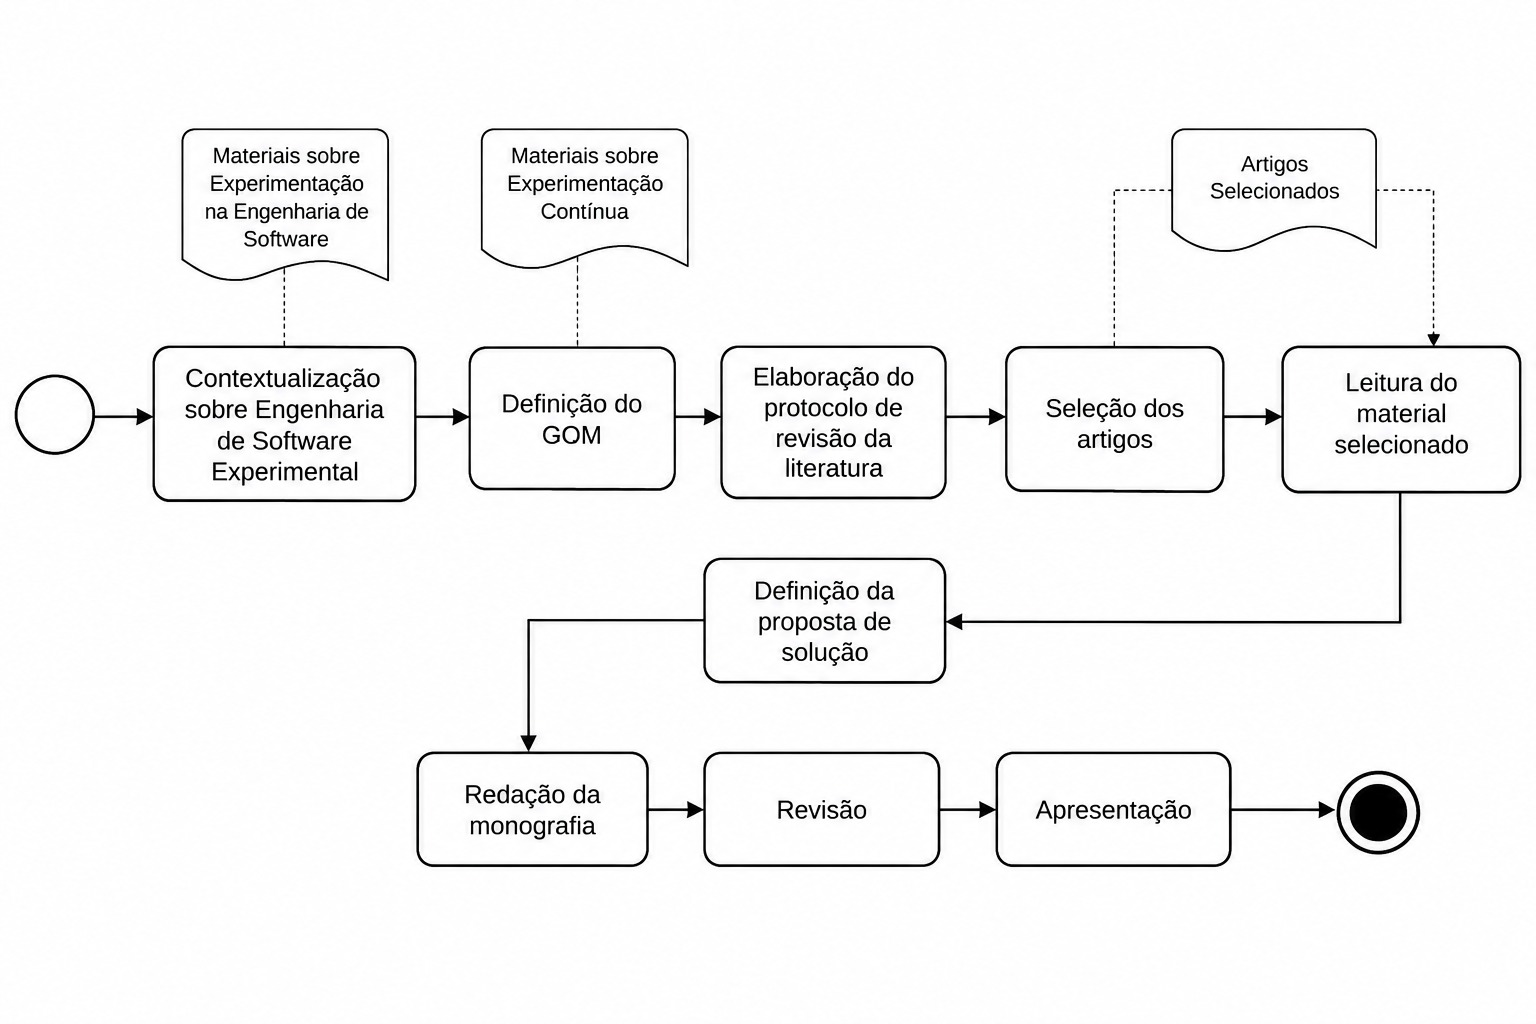
\includegraphics[width=0.8\textwidth]{figuras/fluxo-atividade.png}
    \fonte{Autor (2026).}
\end{figure}

\begin{figure}[H]
    \centering
    \caption{Cronograma realizado na primeira etapa da monografia}
    \label{fig:cronograma-etapa1}
    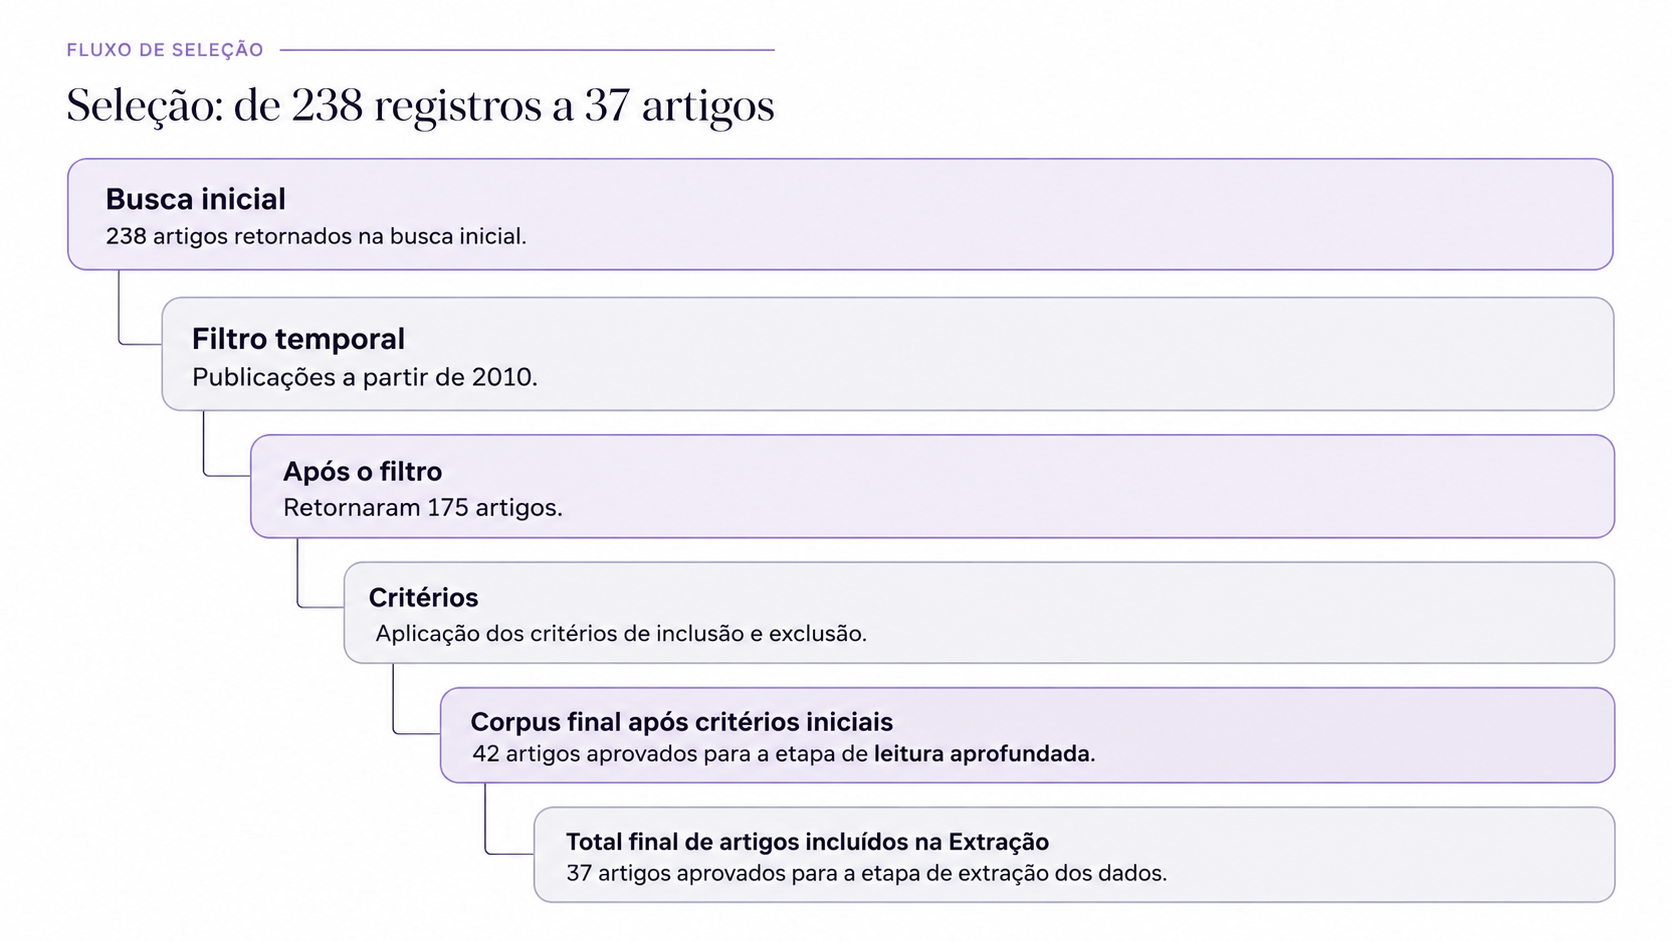
\includegraphics[width=0.8\textwidth]{figuras/selecao-artigos.png}
    \fonte{Autor (2026).}
\end{figure}

As atividades desenvolvidas durante a primeira etapa são descritas a seguir:

\begin{itemize}[
    noitemsep,
    topsep=3pt,
    parsep=0pt,
    partopsep=0pt,
    leftmargin=1.25cm
]
    \item \textbf{Contextualização em Testes de Software e Teste de Mutação:} leituras com o intuito de compreender testes automatizados de aplicações web, cobertura de código e teste de mutação, bem como a abordagem científica necessária para a realização da revisão da literatura;

    \item \textbf{Definição dos Objetivos e Protocolo de Pesquisa:} definição do protocolo de revisão da literatura e dos objetivos da pesquisa segundo a abordagem GQM \cite{basili1994}, da questão de pesquisa norteadora e das questões secundárias; formulação do protocolo da revisão conforme proposto por \citeonline{kitchenham2007}: estratégia PICO, critérios de inclusão e exclusão e formulário de extração de dados;

    \item \textbf{Busca e Seleção dos Estudos:} realização da busca por meio da string de busca elaborada com base na estratégia PICO, seguida da seleção dos estudos conforme os critérios de inclusão e exclusão previamente estabelecidos;

    \item \textbf{Leitura do Material Selecionado e Extração de Dados:} leitura dos estudos selecionados e preenchimento do formulário de extração, com o objetivo de compreender o estado da arte e identificar lacunas, em especial na aplicação do teste de mutação a aplicações web;

    \item \textbf{Definição da Proposta da Solução:} consolidação dos resultados obtidos a partir das questões secundárias e estruturação da abordagem proposta, incluindo a seleção da ferramenta, dos operadores de mutação e das aplicações web a serem avaliadas, bem como a definição de estratégias para redução de custos;

    \item \textbf{Escrita do Trabalho:} redação da monografia seguindo a organização apresentada na Seção~\ref{sec:organizacao-trabalho};

    \item \textbf{Revisão da Monografia:} revisão e correção; e

    \item \textbf{Apresentação do Trabalho:} apresentação da primeira parte desta monografia para a banca avaliadora.
\end{itemize}

\subsection{Segunda Etapa}


Esta subseção apresenta as atividades previstas para a segunda etapa desta monografia, que compreende a aplicação da abordagem proposta por meio da mineração de repositórios de software (\textit{Repository Mining}), a execução dos testes de mutação e a análise dos resultados obtidos. As atividades serão organizadas em um fluxo de execução e distribuídas em um cronograma.

\begin{figure}[H]
    \centering
    \caption{Fluxo de atividades da segunda etapa da monografia}
    \label{fig:exemplo}
    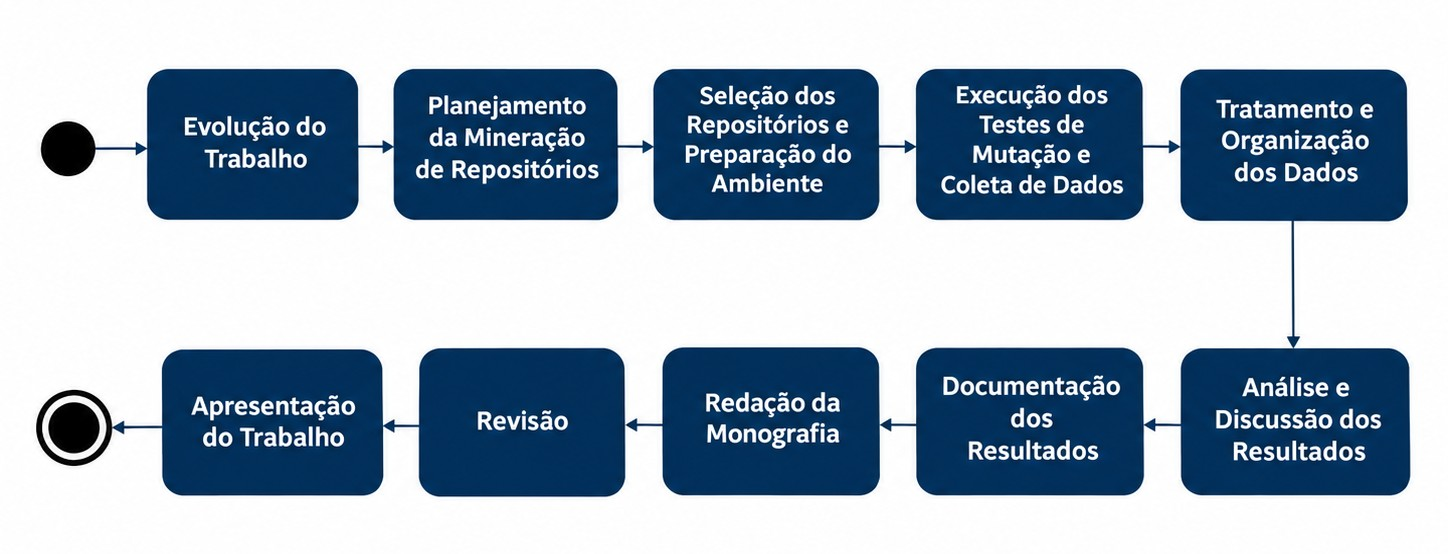
\includegraphics[width=0.8\textwidth]{figuras/Fluxo-de-Atividades-da-Monografia.png}
\end{figure}
  \fonte{Autor (2026).}

\begin{itemize}[noitemsep, topsep=0pt]

    \item \textbf{Evolução do Trabalho:} revisão e aprimoramento do material desenvolvido na primeira etapa, considerando as observações e recomendações da banca avaliadora, bem como os ajustes necessários à proposta de solução;

    \item \textbf{Planejamento da Mineração de Repositórios:} definição dos critérios de inclusão e exclusão para a seleção de repositórios de aplicações web de código aberto, considerando características como linguagem de programação, disponibilidade de suítes de testes automatizados e viabilidade de execução dos testes de mutação. Também serão definidas as unidades de análise, as fontes de dados e os procedimentos de extração \cite{acmsigsoft};

    \item \textbf{Seleção dos Repositórios e Preparação do Ambiente:} identificação e seleção dos repositórios conforme os critérios estabelecidos, seguida da configuração dos ambientes e das ferramentas necessárias para a execução das suítes de testes e aplicação dos operadores de mutação;

    \item \textbf{Execução dos Testes de Mutação e Coleta de Dados:} aplicação dos operadores de mutação ao código-fonte das aplicações selecionadas e execução das respectivas suítes de testes automatizados. Serão coletados dados referentes à quantidade de mutantes gerados, mortos e sobreviventes, ao \textit{Mutation Score}, à cobertura de código e ao tempo de execução;

    \item \textbf{Tratamento e Organização dos Dados:} processamento, validação e consolidação dos dados obtidos, considerando a identificação de execuções inválidas, possíveis mutantes equivalentes e demais fatores que possam comprometer a interpretação dos resultados;

    \item \textbf{Análise e Discussão dos Resultados:} análise quantitativa dos indicadores coletados para avaliar a eficácia das suítes de testes na detecção das alterações introduzidas artificialmente. Serão investigados os fatores associados à sobrevivência dos mutantes, as relações entre cobertura de código e \textit{Mutation Score}, bem como as limitações e ameaças à validade da investigação. Os resultados serão discutidos à luz das evidências identificadas na revisão da literatura;

    \item \textbf{Documentação dos Resultados:} apresentação dos procedimentos realizados e dos resultados obtidos com a mineração dos repositórios, buscando responder à questão principal de pesquisa e avaliar as contribuições e limitações da abordagem proposta;

    \item \textbf{Redação e Revisão da Monografia:} continuidade da escrita do trabalho, conforme a estrutura apresentada na Seção, seguida da revisão e correção do documento em conjunto com o orientador; e

    \item \textbf{Apresentação do Trabalho Finalizado:} preparação e apresentação da versão final da monografia à banca avaliadora.

\end{itemize}